\documentclass{beamer}  
\usepackage[UTF8,noindent]{ctex} 
\usetheme{CambridgeUS}
\usecolortheme{rose} 

%固定图片位置,使用参数H
\usepackage{float}

% Windows系统使用
%\usepackage{xeCJK}
%\setCJKmainfont{SimSun}

% Mac系统使用
\usepackage{xeCJK}
\setCJKmainfont[BoldFont=STHeiti,ItalicFont=STKaiti]{STSong}
\setCJKsansfont[BoldFont=STHeiti]{STXihei}
\setCJKmonofont{STFangsong}

%为制作幻灯片设计的无衬线字体包,对正文字体和数学字体都有详细的调整
\usepackage{arev}

\title[曲面偏微分方程数值解]{Beamer幻灯片} 
\subtitle[ppt篇]{Slide} 
\author{quxk}
%\institute{}

%自定义时间
%\date[06/13/17]{2017年6月13日} 

%系统时间
\date{\small \today \ \\ {\it}}

%隐藏时间
%\date{}

\institute[LSEC]{中国科学院大学} 

\begin{document}

%生成主页
\begin{frame} 
	\titlepage 
\end{frame} 
    
%\begin{frame}
%	\maketitle
%\end{frame}


%生成目录
\begin{frame}
\frametitle{Outline}
\tableofcontents
\end{frame}


\section{Introduction}
\begin{frame}
\frametitle{Introduction\_1}
内容.
\end{frame}

\begin{frame}
\frametitle{Introduction\_2}
\begin{block}{勾股定理及巴塞尔问题}
\begin{align*}
\sqrt{a^2 + b^2} &= c^2,\\
\sum_{n=1}^\infty \frac1{n^2}&=\frac{\pi^2}6.
\end{align*}
\end{block}
\end{frame}


\section{Finite Element Methods}
\begin{frame}
\frametitle{Finite Element Methods\_1}
FEM 方法
\end{frame}

\begin{frame}
\frametitle{Finite Element Methods\_2}
弱形式
\end{frame}

\section{Error}
\begin{frame}
\frametitle{Error\_1}
L2误差
\end{frame}

\begin{frame}
\frametitle{Error\_2}
H1误差
\begin{figure}[h!t!b]
	\centering	
	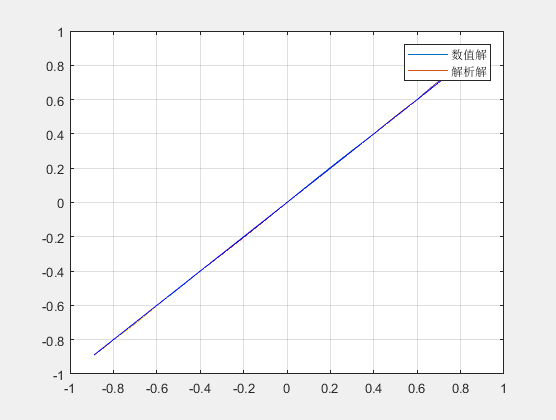
\includegraphics[height=0.4\linewidth]{./pictures/040.png}
	\caption{h=0.05,Test space $V=H^1_0$}\label{fig:1}
\end{figure}
\end{frame}



\begin{thebibliography}{99}
\bibitem{Braess} Braess  Finite Elements
\bibitem{shu} 刘海洋《\LaTeX 入门》
\end{thebibliography}



\end{document}